\documentclass{beamer}

\usepackage{beamerthemesplit}
\usepackage{verbatim}
\usepackage[normalem]{ulem}

\usepackage{xcolor}

\usepackage{hyperref}

\definecolor{gold}{rgb}{1.,0.84,0.}
\definecolor{brightred}{rgb}{1.,0.4,0.4}
\definecolor{mygray}{RGB}{200,200,200}
\definecolor{lightsteelblue}{RGB}{176,196,222}
\definecolor{lightskyblue}{RGB}{135,206,250}
\definecolor{cadetblue}{RGB}{95,158,160}

\usetheme{default}
\usecolortheme{mule}

\usefonttheme{serif}

%\DeclareGraphicsExtensions{.pdf,.png,.jpg}

\newcommand{\mcal}{\textsc{metacalibration}}
\newcommand{\Mcal}{\textsc{Metacalibration}}

\newcommand{\mcalR}{\mbox{\boldmath $R$}}
\newcommand{\mcalRscalar}{\mbox{$R$}}

\newcommand{\mcalRmean}{\mbox{\boldmath $\langle R \rangle$}}
\newcommand{\mcalRscalarmean}{\mbox{$\langle R \rangle$}}

\newcommand{\mcalRpsf}{$R^{p}$}
\newcommand{\mcalRpsfnoise}{$R^{p}_\eta$}
\newcommand{\mcalRo}{\mbox{\boldmath $R_o$}}
\newcommand{\mcalRnoise}{\mbox{\boldmath $R_\eta$}}

\newcommand{\mcalRmeanalpha}{\mbox{\boldmath $\langle R_\alpha \rangle$}}
\newcommand{\mcalRmeanbeta}{\mbox{\boldmath $\langle R_\beta \rangle$}}

\newcommand{\mcalRg}{\mbox{\boldmath $R_\gamma$}}
\newcommand{\mcalRS}{\mbox{\boldmath $R_S$}}
\newcommand{\mcalRgmean}{\mbox{\boldmath $\langle R_\gamma \rangle$}}
\newcommand{\mcalRSmean}{\mbox{\boldmath $\langle R_S \rangle$}}

\newcommand{\mcalRtwopt}{\mbox{\boldmath $R^{2pt}$}}
\newcommand{\mcalRtwoptmean}{\mbox{\boldmath $\langle R^{2pt} \rangle$}}


\newcommand{\mcalRmodel}{\mbox{\boldmath $R^{model}$}}
\newcommand{\mcalRnoisemodel}{\mbox{\boldmath $R^{model}_\eta$}}


\newcommand{\vecg}{\mbox{\boldmath $\gamma$}}
\newcommand{\vest}{\mbox{\boldmath $e$}}

\newcommand{\snr}{$S/N$}
\newcommand{\snT}{$(S/N)_{\textrm{size}}$}
%\newcommand{\snT}{$\left( \frac{S}{N}\right)_{\textrm{size}}$}
\newcommand{\snflux}{$(S/N)_{\textrm{flux}}$}
%\newcommand{\snflux}{$\left( \frac{S}{N}\right)_{\textrm{flux}}$}

\newcommand{\lensfit}{\texttt{LENSFIT}}
\newcommand{\numba}{\texttt{Numba}}
\newcommand{\python}{\texttt{Python}}
\newcommand{\ngmix}{\texttt{ngmix}}
\newcommand{\shear}{{\bf g}}
\newcommand{\redmapper}{redMaPPer}
\newcommand{\est}{$e$}


\newcommand{\prelim}{{\bf{\it Preliminary}}}



\title{The Effect of Blended Objects on \mcal}
\author{Erin Sheldon}
\institute{Brookhaven National Laboratory}

% http://texblog.net/latex-archive/plaintex/beamer-footline-frame-number/
% to add the page (frame ) number and not screw up the bottom line
% works for split themes?
\expandafter\def\expandafter\insertshorttitle\expandafter{%
      \insertshorttitle\hfill%
        \insertframenumber\,/\,\inserttotalframenumber}

% suppress navigation bar
\beamertemplatenavigationsymbolsempty
\setbeamertemplate{footline}{}

\begin{document}

\frame{\titlepage}


\setbeamertemplate{background canvas}[vertical shading][bottom=mgray,top=mblack]

\frame
{
    \frametitle{Outline}

    \setbeamerfont*{itemize/enumerate body}{size=\Large}
    \setbeamerfont*{itemize/enumerate subbody}{parent=itemize/enumerate body}
    \setbeamerfont*{itemize/enumerate subsubbody}{parent=itemize/enumerate body}
 
    \begin{itemize}

        \item Blended Objects
        \item Simulations
        \item Preliminary Results

    \end{itemize}

}

\frame
{
    \frametitle{Blended Objects}

    \setbeamerfont*{itemize/enumerate body}{size=\large}
    \setbeamerfont*{itemize/enumerate subbody}{parent=itemize/enumerate body}
    \setbeamerfont*{itemize/enumerate subsubbody}{parent=itemize/enumerate body}
 
    \begin{itemize}

        \item In DES we identified blending as the most important systematic
            for shear estimation.

        \item Blending is the scenario where the images of multiple objects overlaps
            on the sky.

        \item Blending can occur for objects that are physically associated, or
            for chance projections 

            \begin{itemize}
                \item Faint galaxies that are below the detection threshold are counted
                    as part of the galaxy or part of the background
            \end{itemize}

        \item Can concievably cause instability in the model fitting algorithm, which
            may cause errors in the shear calibration.

        \item More importantly, can cause biases in redshift determination:
            beyond the scope of this project. 


    \end{itemize}

}


{

    \frame
    {
     
        \begin{center}
            \includegraphics[width=0.8\textwidth]{hdf_hogg.jpg}
            \newline
        \end{center}

    }
    \setbeamertemplate{background canvas}[vertical shading][bottom=mgray,top=mblack]

}


\frame
{
    \frametitle{Simulations}

    \setbeamerfont*{itemize/enumerate body}{size=\large}
    \setbeamerfont*{itemize/enumerate subbody}{parent=itemize/enumerate body}
    \setbeamerfont*{itemize/enumerate subsubbody}{parent=itemize/enumerate body}
 
    \begin{itemize}


        \item Take size and flux distribution from {\color{brightred}COSMOS}, depth {\color{gold} $i=25.2$}

        \item ``Fake'' the fainter galaxies to {\color{gold}$i \sim 27.5$} by
            scaling galaxy flux.  Also scale down the sizes.   Add some stars and very
            big bright galaxies as well.

        \item Noise level appropriate for DES: detection threshold approximately
            {\color{lightskyblue} $i=24.1$}

        \item Galaxies placed randomly on the sky.

        \item Two different source planes, with shears {\color{gold}$\gamma_1 = 0.01$}
            and {\color{gold} $\gamma_2 = 0.02$}


    \end{itemize}

}


{

    \frame
    {
        \frametitle{Example Simulation}
     
        \begin{center}
            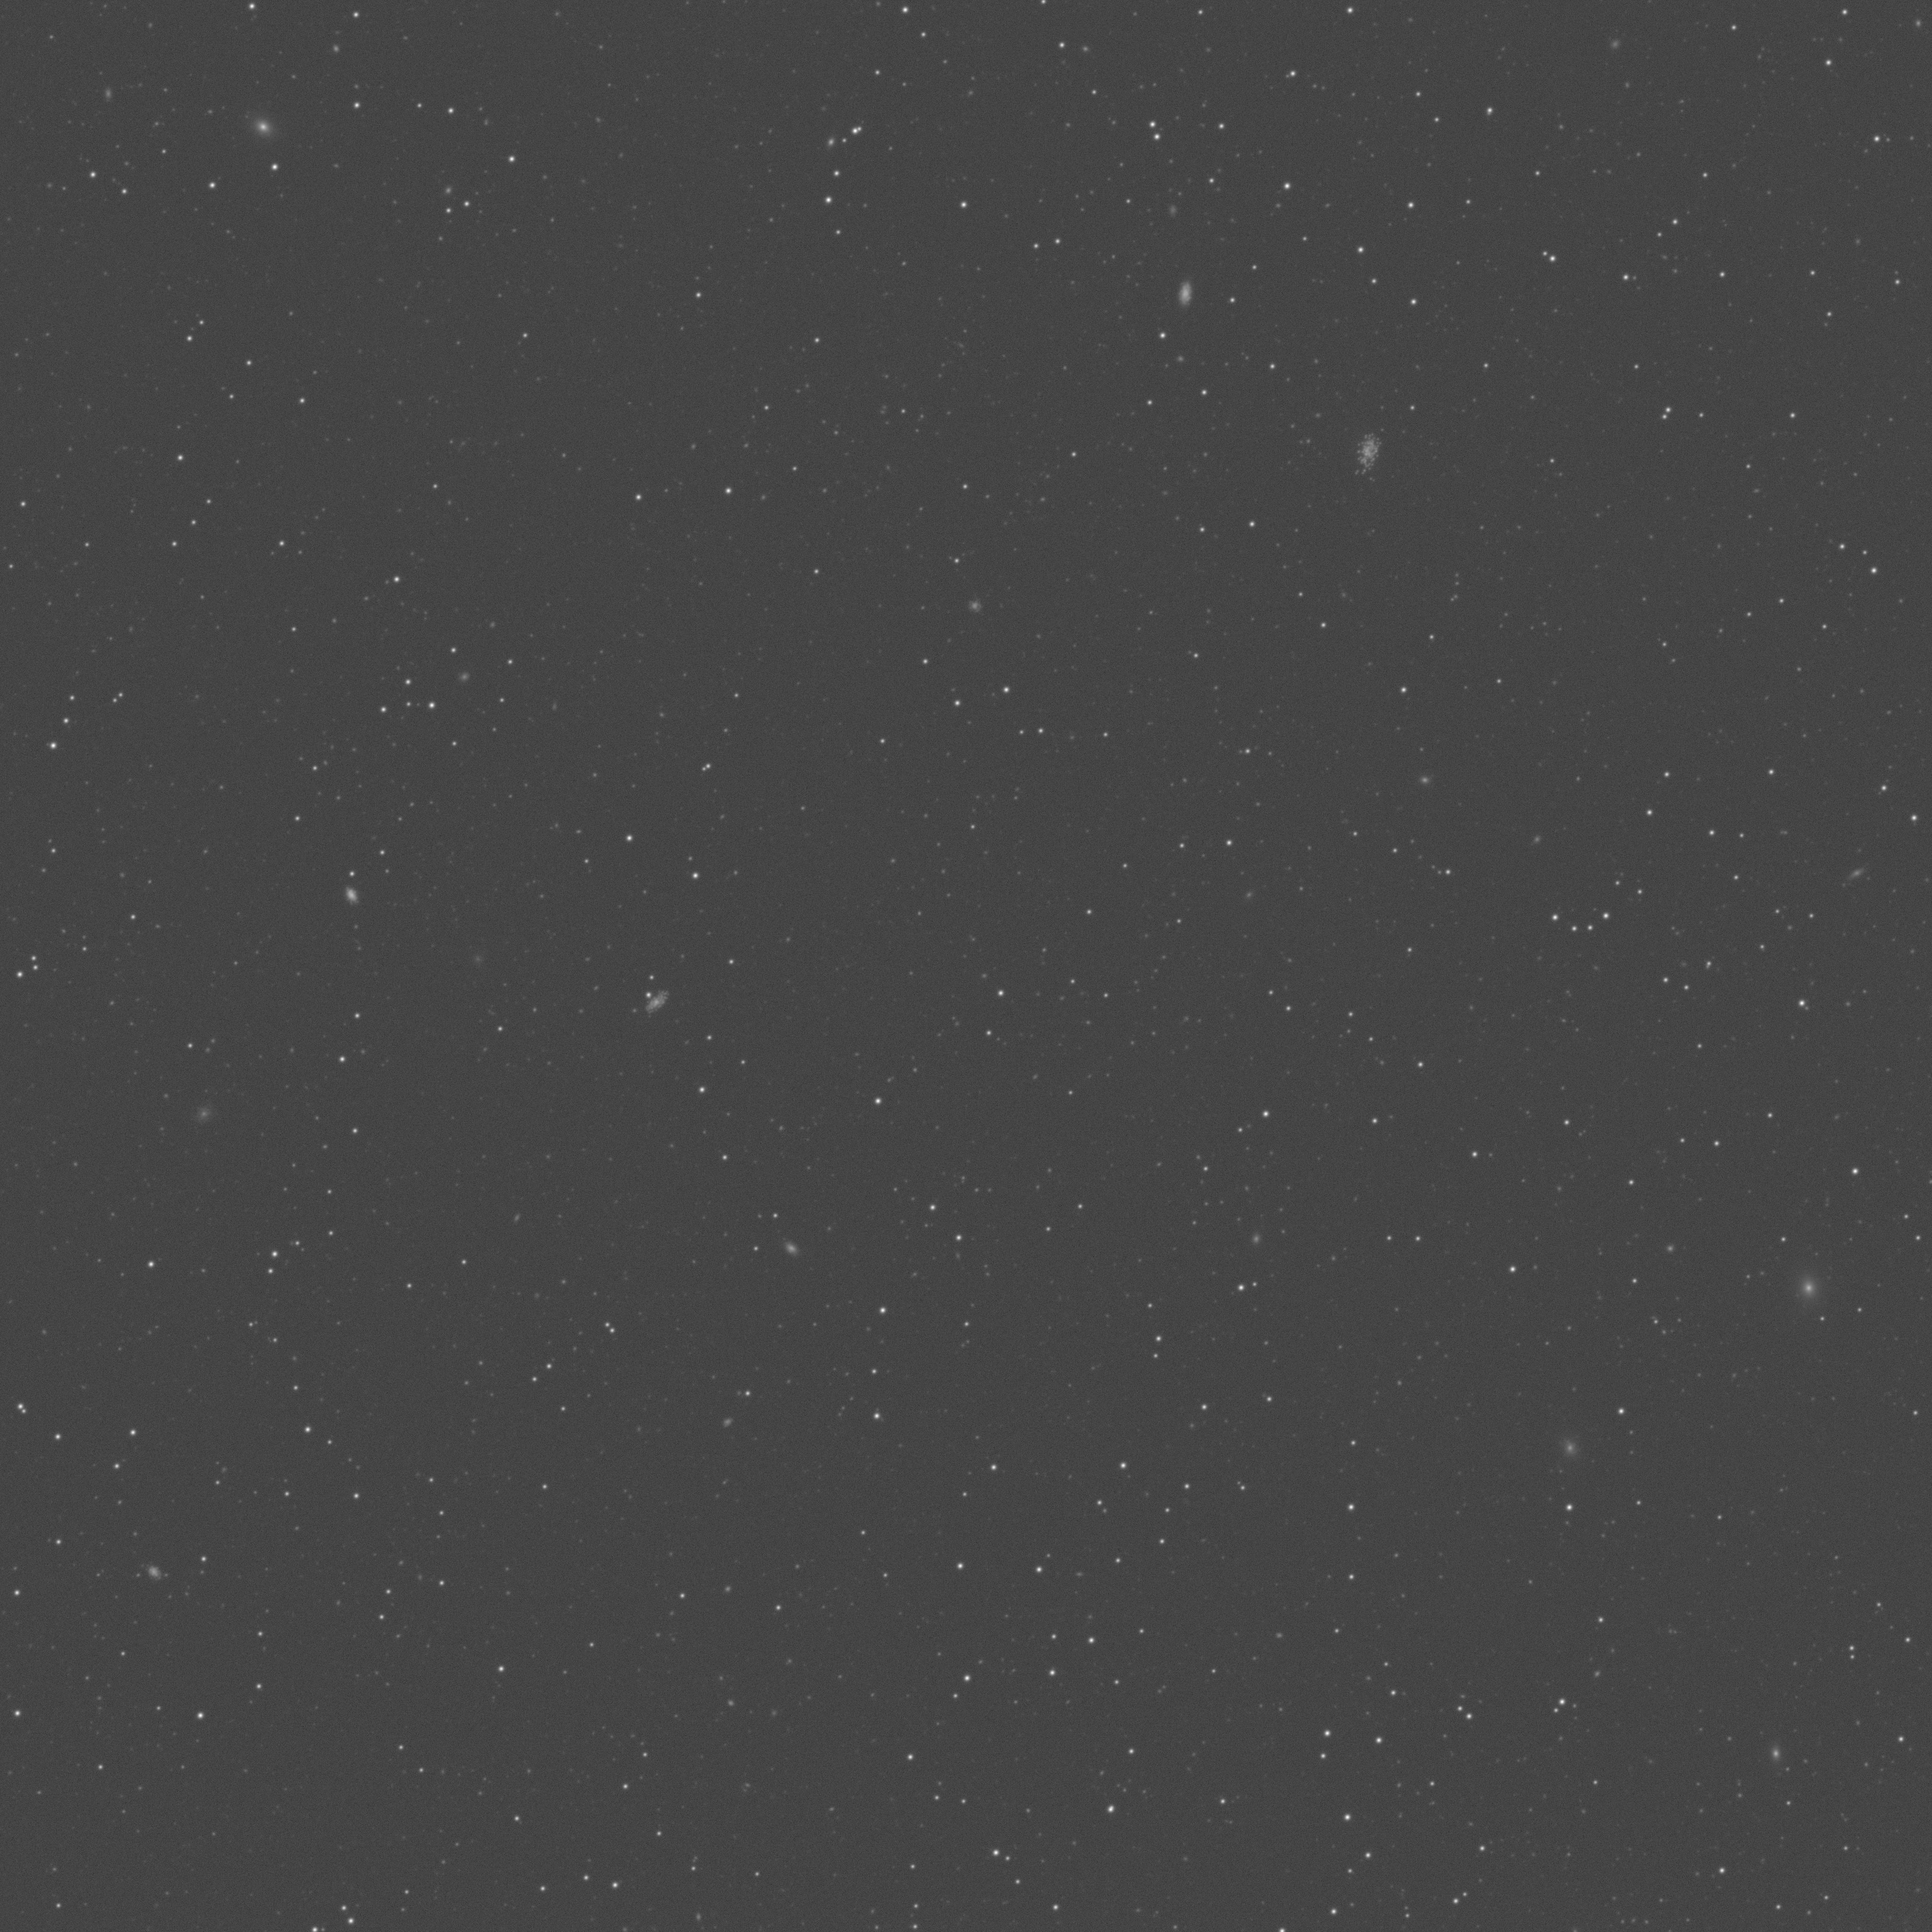
\includegraphics[width=0.8\textwidth]{nbrsim-003e-000023-image.jpg}
            \newline
        \end{center}

    }
    \setbeamertemplate{background canvas}[vertical shading][bottom=mgray,top=mblack]

}

{

    \frame
    {
        \frametitle{Example Simulation}
     
        \begin{center}
            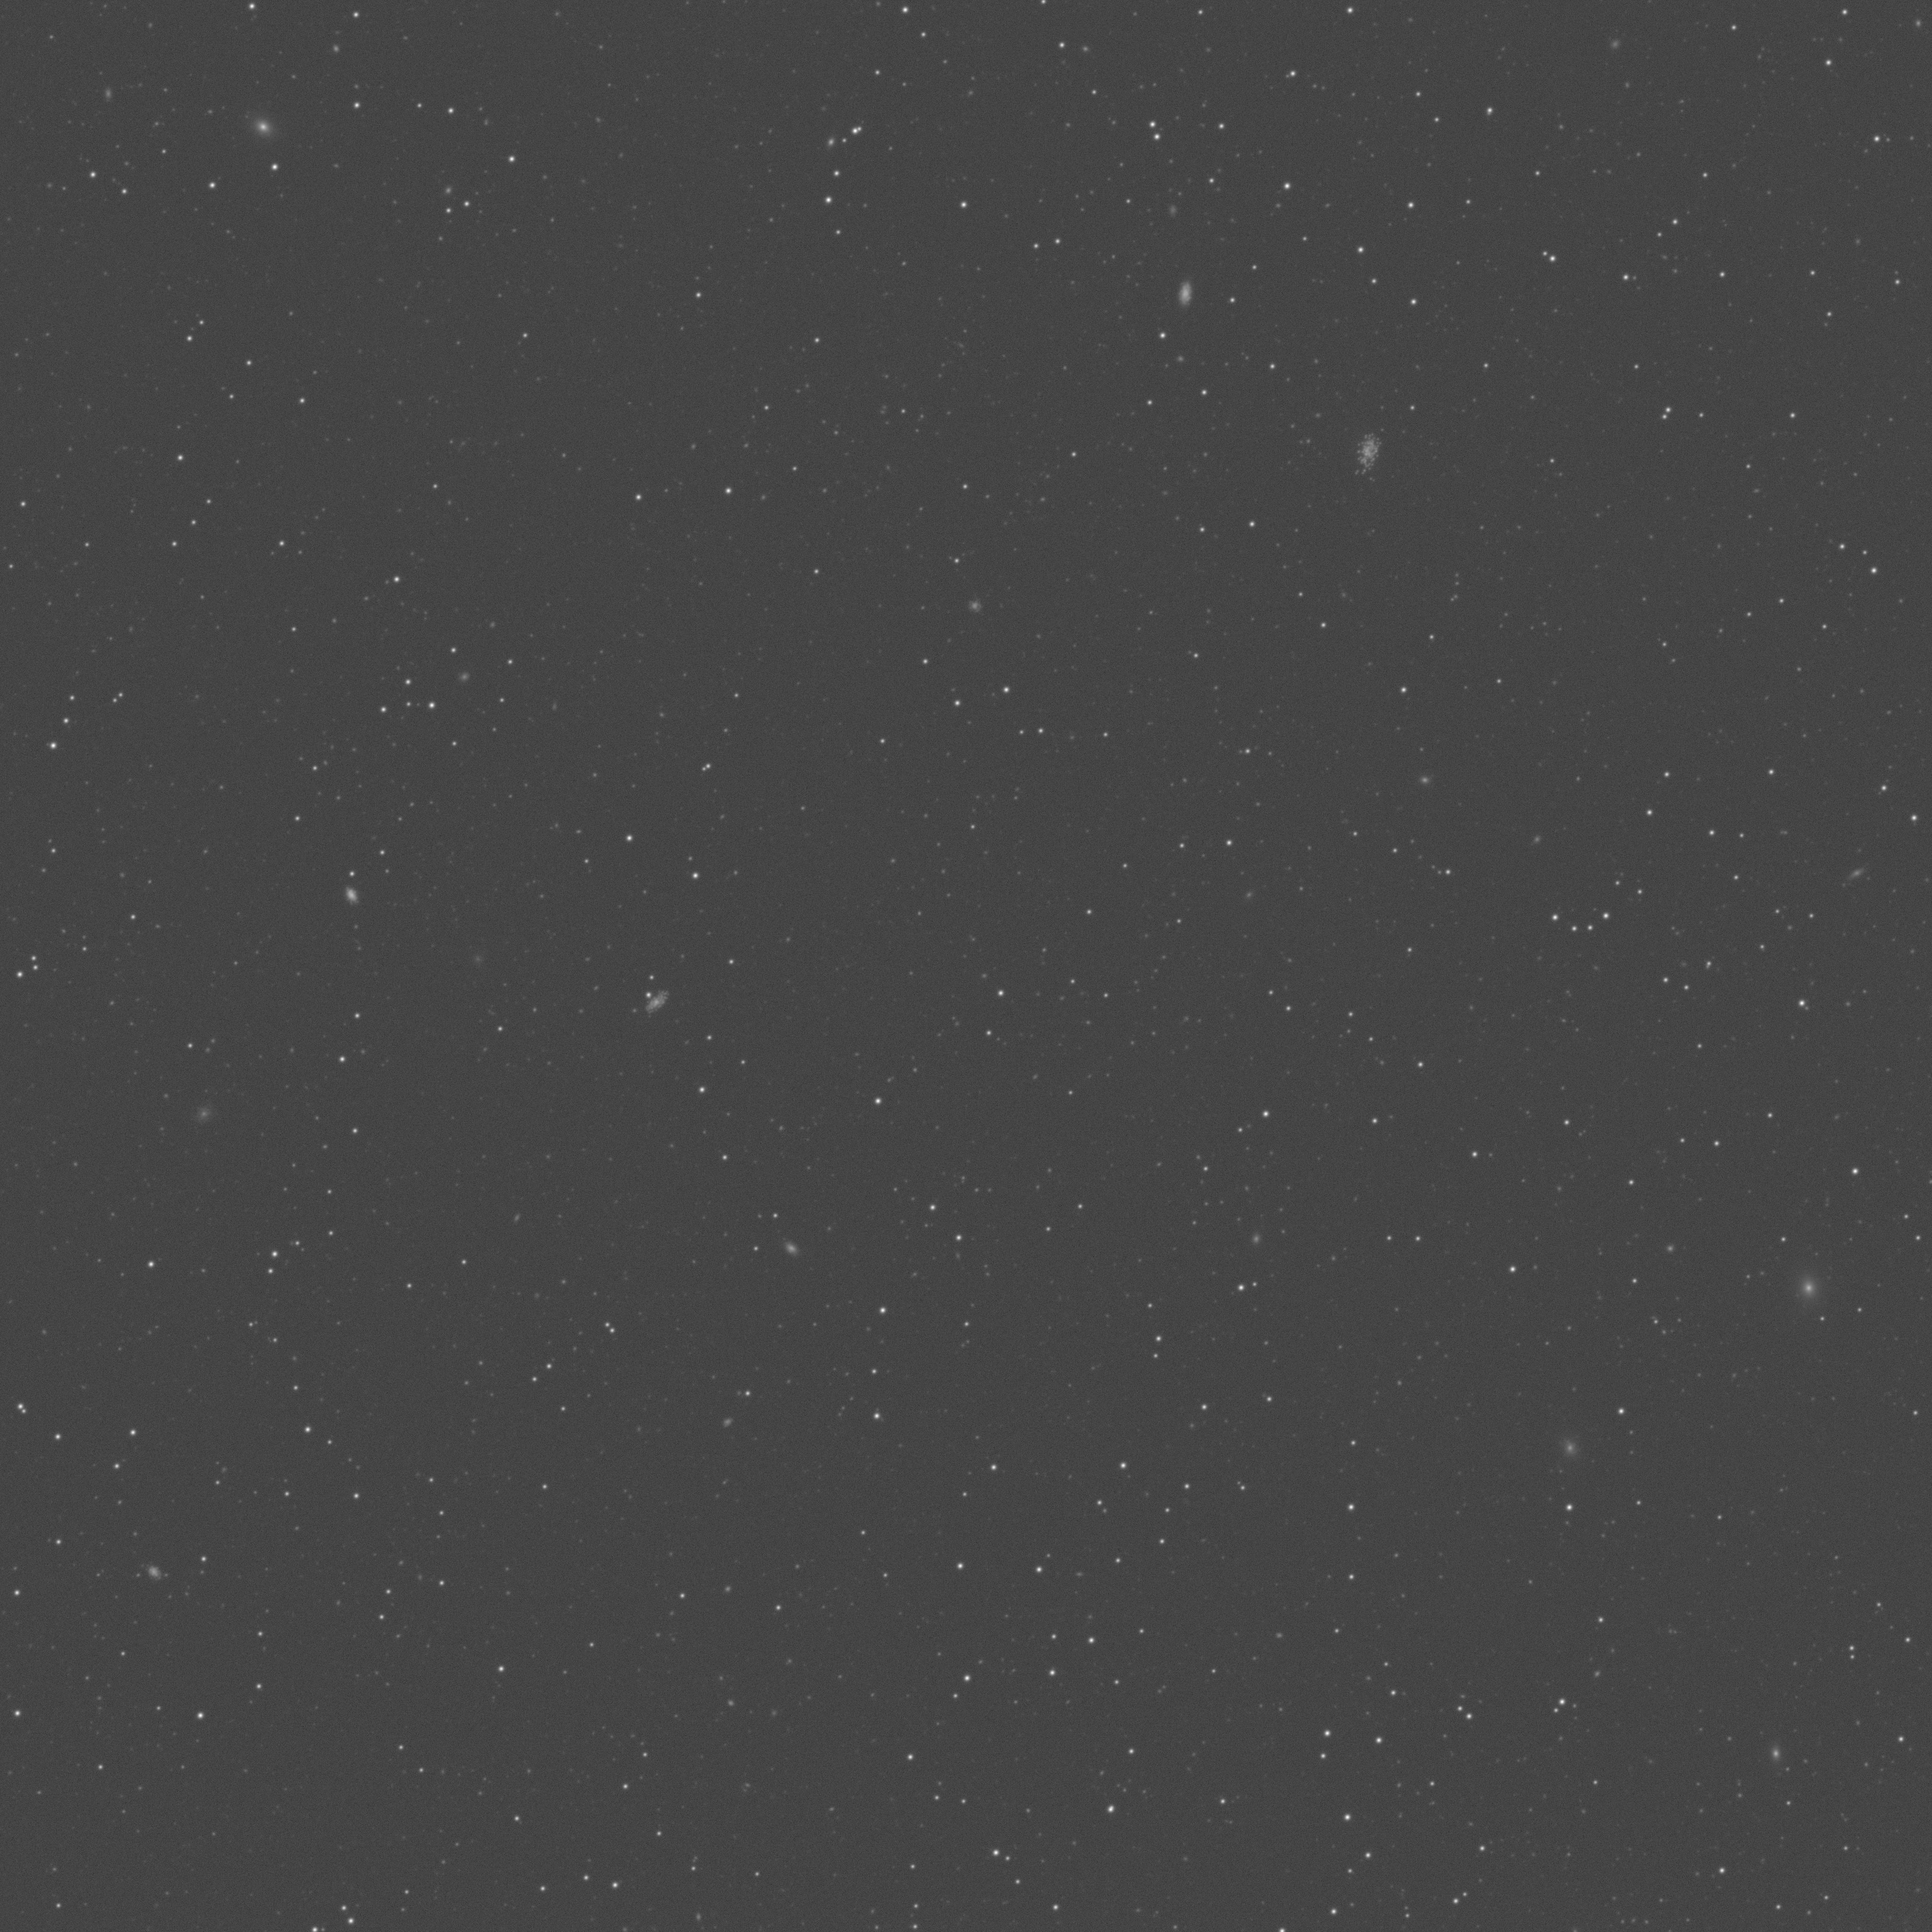
\includegraphics[width=1.6\textwidth]{nbrsim-003e-000023-image.jpg}
            \newline
        \end{center}

    }
    \setbeamertemplate{background canvas}[vertical shading][bottom=mgray,top=mblack]

}

{

    \frame
    {
        \frametitle{Example Simulation}
     
        \begin{center}
            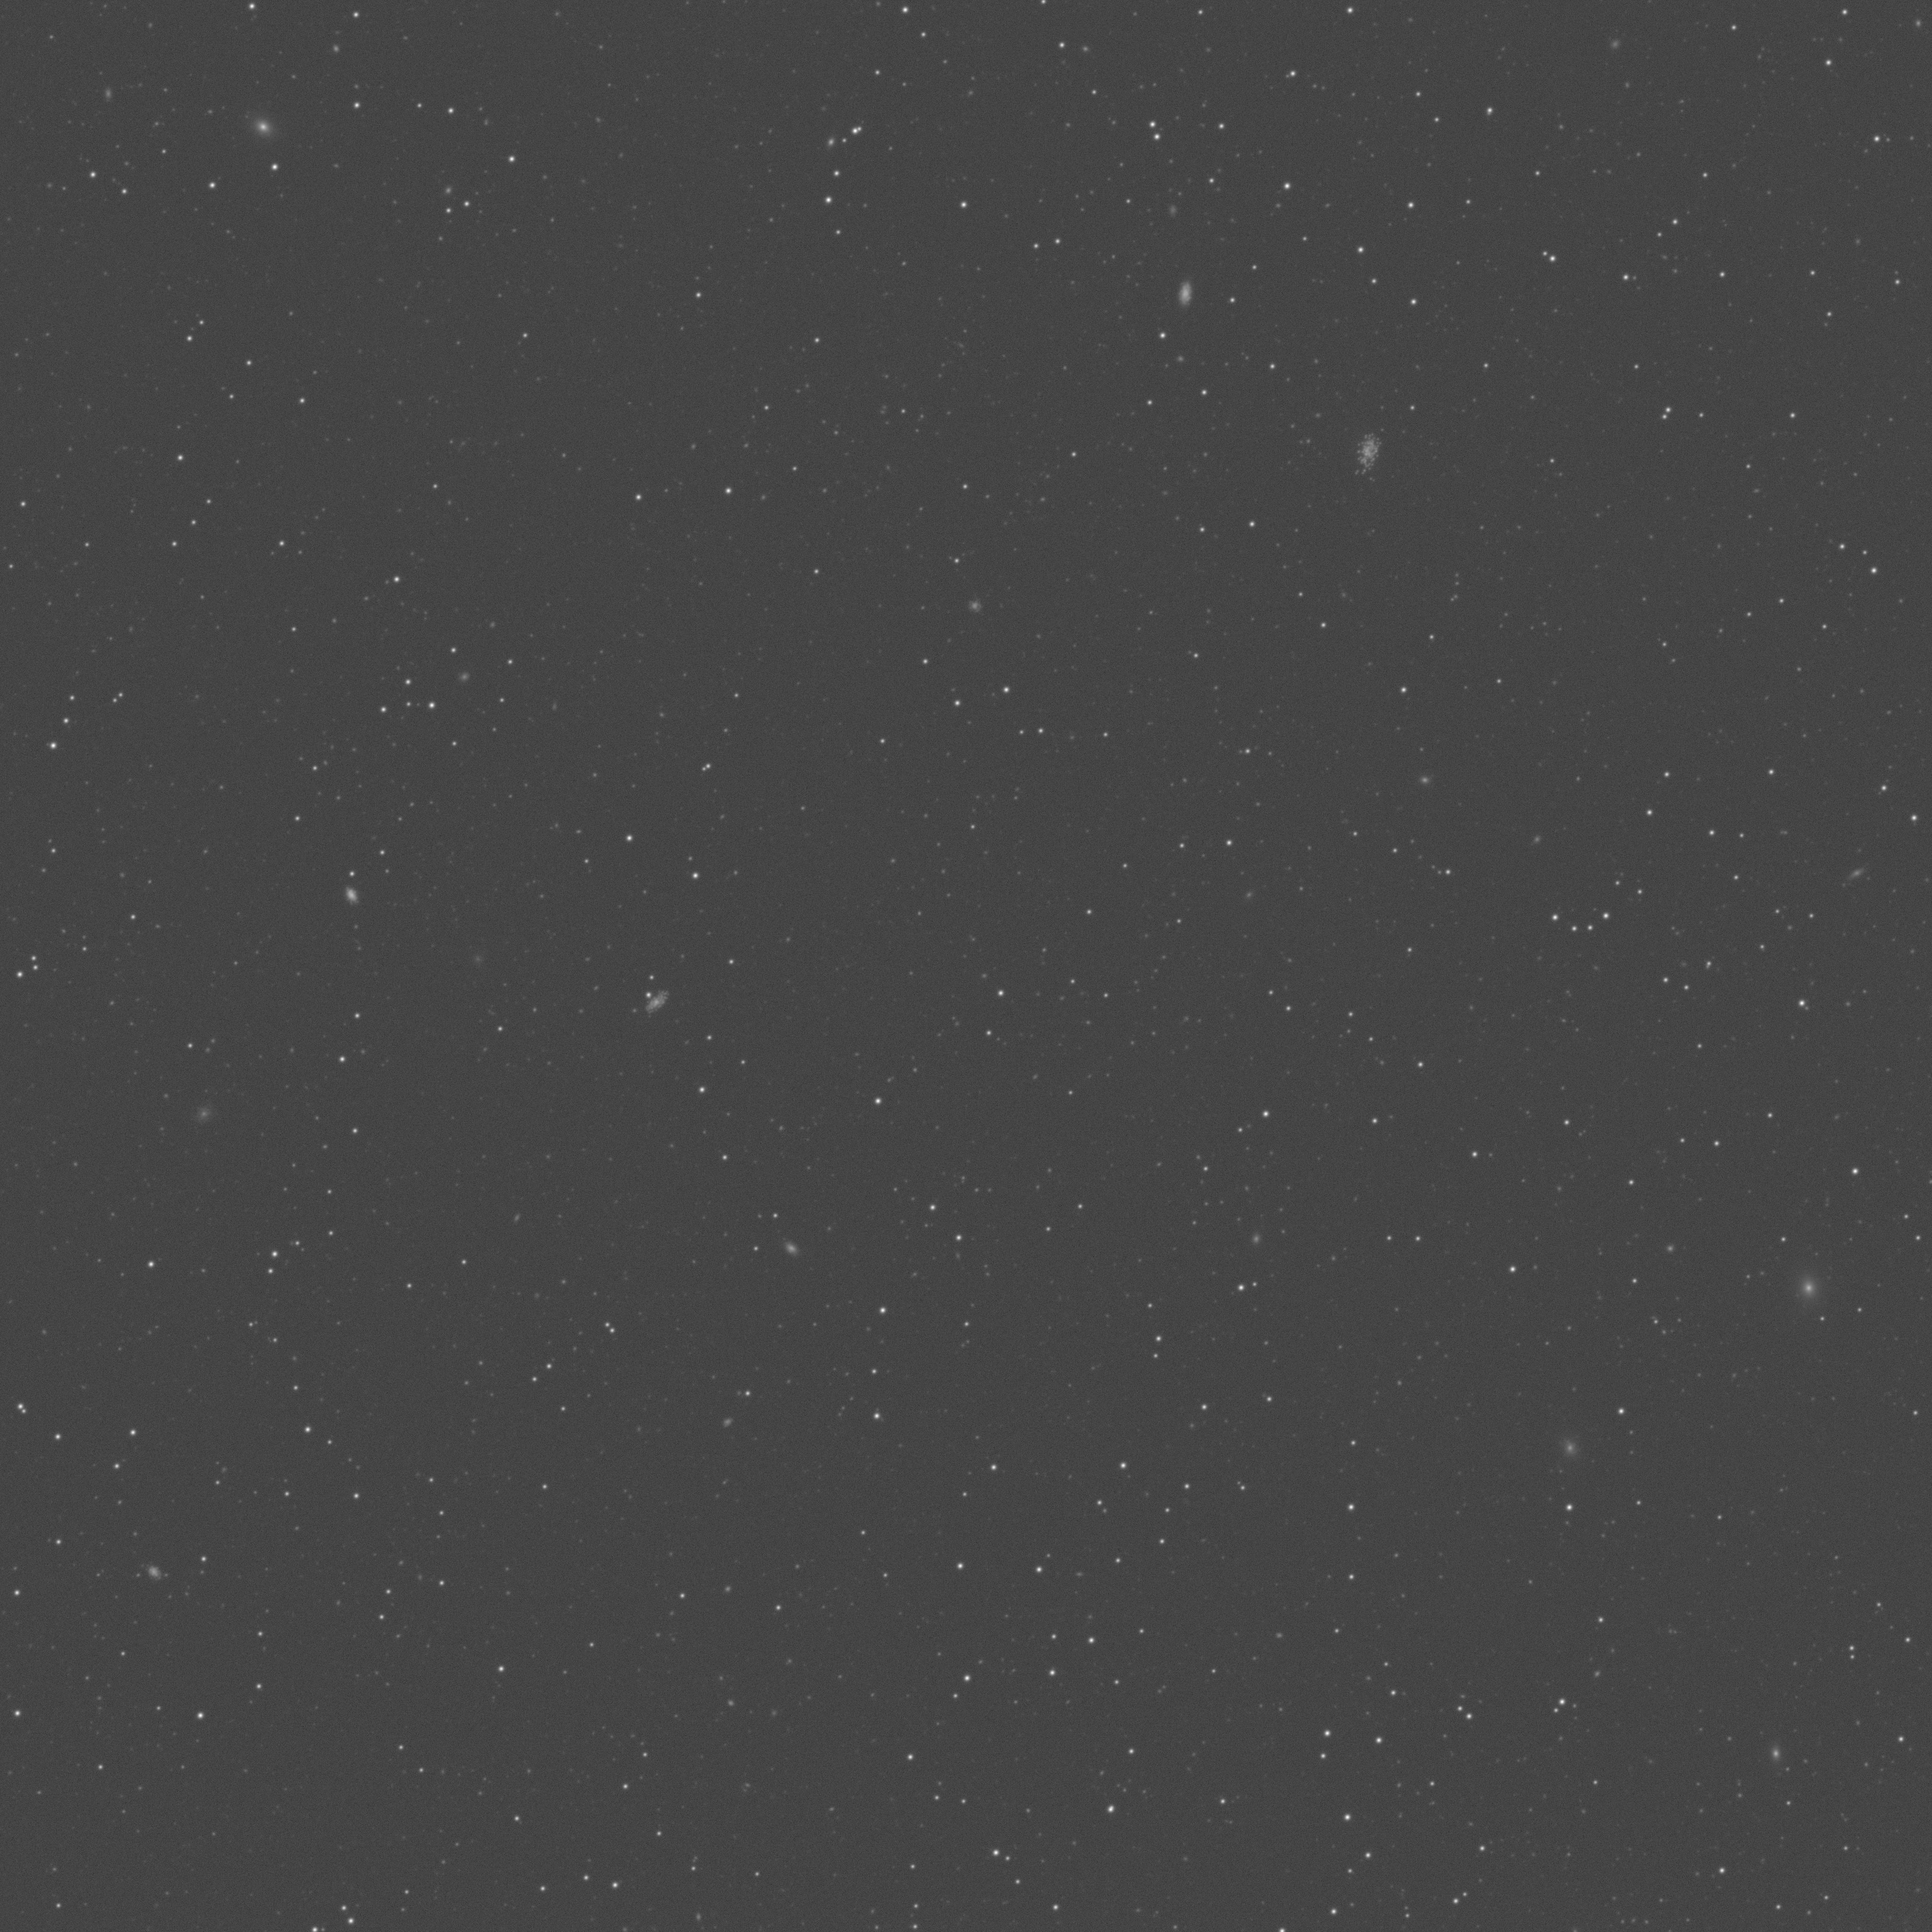
\includegraphics[width=2.5\textwidth]{nbrsim-003e-000023-image.jpg}
            \newline
        \end{center}

    }
    \setbeamertemplate{background canvas}[vertical shading][bottom=mgray,top=mblack]

}


\frame
{
    \frametitle{Preliminary Results: Multiplicative Bias $m$}

    \setbeamerfont*{itemize/enumerate body}{size=\large}
    \setbeamerfont*{itemize/enumerate subbody}{parent=itemize/enumerate body}
    \setbeamerfont*{itemize/enumerate subsubbody}{parent=itemize/enumerate body}
 
    \begin{itemize}

        \item Masking the light from neighbors (see Jarvis, Sheldon et al. 2015)

        \item Errors are 95\% confidence

        \item $S/N > 10$ $m: +(4.6 \pm 3.9) \times 10^{-3}$

        \item $S/N > 15$ $m: -(0.6 \pm 4.1) \times 10^{-3}$

        \item $S/N > 20$ $m: +(1.1 \pm 4.6) \times 10^{-3}$

    \end{itemize}

}


\frame
{
    \frametitle{Future Work}

    \setbeamerfont*{itemize/enumerate body}{size=\large}
    \setbeamerfont*{itemize/enumerate subbody}{parent=itemize/enumerate body}
    \setbeamerfont*{itemize/enumerate subsubbody}{parent=itemize/enumerate body}
 
    \begin{itemize}


        \item Get more statistics

        \item Run in a mode where neighbor light is subtracted.

    \end{itemize}

}




\end{document}
